\section{Arquitetura de Software}
\label{sec:arquitetura-software}

A arquitetura GNC, demonstrada pela Figura 7, tem objetivo de explicar a relação entre os componentes de cada um desses sistemas, assim como explicar o funcionamento e comportamento de todo o sistema. Apesar de ter esse nome, também estão inclusos um componente de GUI e um de comunicação no diagrama, mas são a minoria dos componentes. Mesmo que sejam a menor parte da arquitetura, não significa que não são trabalhosos para desenvolver. Essa arquitetura também possui o agrupamento por estruturas físicas, porém nesse diagrama só estão representadas as estações de controle, flutuante e o BROV completo. O padrão que se está utilizando é o UML (Unified Modeling Language), no qual o “garfo” representa o componente que faz aquisição da informação e o círculo preenchido representa o componente que fornece a informação.

\begin{figure}[h]
	\centering
	\caption[Arquitetura GNC]{Arquitetura GNC}
	\label{fig:arquitetura-software}
	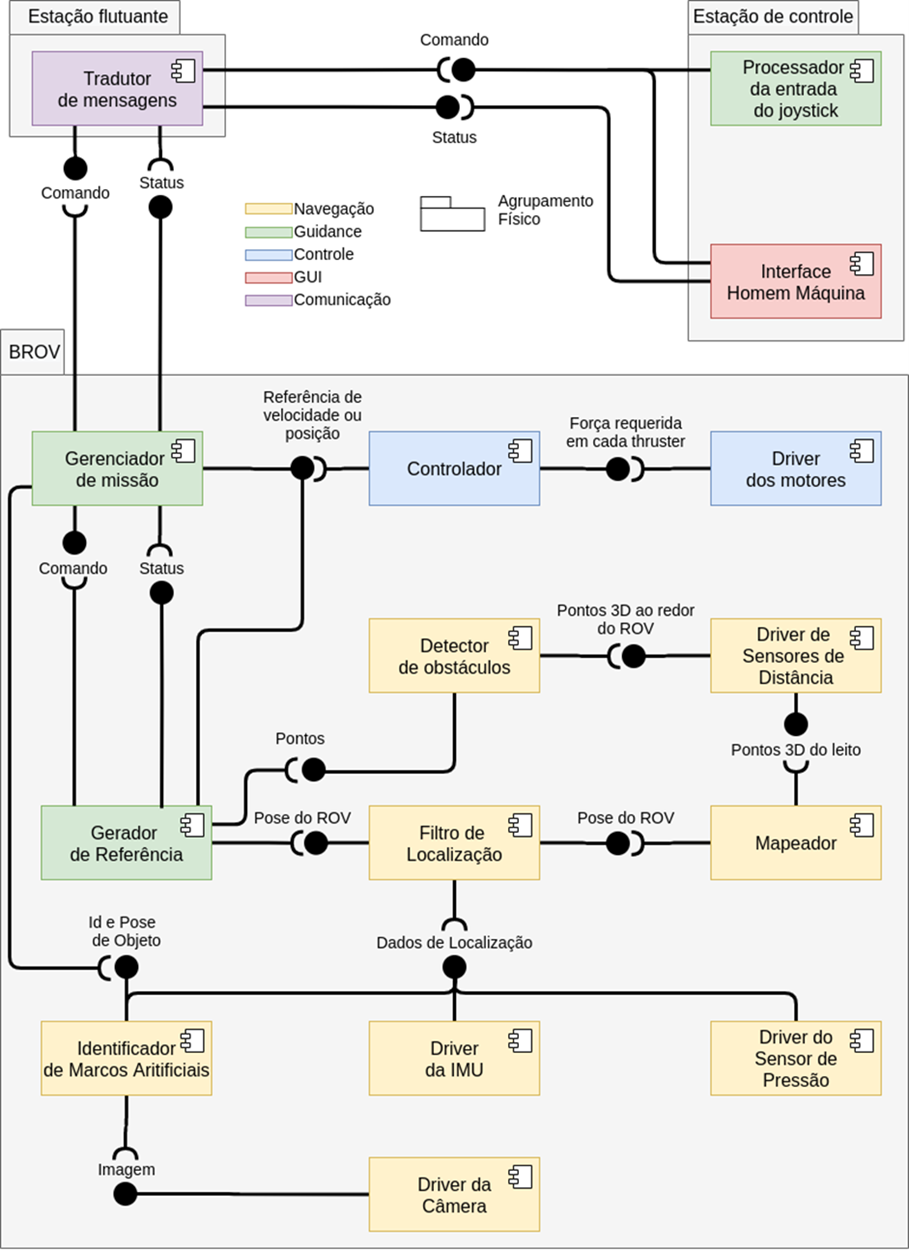
\includegraphics[width=0.9\linewidth]{images/arquitetura-software}\\
	\footnotesize Fonte: Autores
\end{figure}

O trabalho em questão utilizará ROS (Robot Operating System) para programação de cada componente. O ROS é uma ferramenta que facilita comunicação entre programas e encapsula diversas soluções de robótica relacionadas a todos os sistemas definidos nesse trabalho. É importante se entender que toda a arquitetura estará em execução simultaneamente, cada componente, representado por retângulos no UML, troca informações com outros durante em tempo real durante a execução.

Na estação de controle, dois componentes são executados, um de guidance que tem o papel de receber a mensagem do joystick, converter no tipo de dado específico e enviar para o tradutor. O outro componente é de GUI, esse é a tela que o operador irá visualizar e interagir, portanto recebe mensagens do ROV que passam pelo tradutor e envia comandos para o ROV.  Na estação flutuante está um componente de comunicação, responsável por traduzir mensagens do ROV e da estação de controle e enviá-las utilizando o protocolo que ainda será especificado no próximo trabalho.

O BROV contém a maior parte dos componentes do sistema, sendo o gerenciador o responsável por definir o comportamento do ROV. O gerenciador recebe o comando do joystick e da IHM, então conforme a vontade do operador, o ROV pode ser controlado manualmente ou fazer uma missão automaticamente. No caso do controle manual, o gerenciador envia a referência de velocidade nos 4 DOF (surge, sway, heave e yaw) para o controlador, o qual somente calcula a ação de controle, ou seja, o empuxo necessário em cada motor, que é enviada para cada o driver de motores. Os drivers são responsáveis por se comunicarem com os componentes eletrônicos, que são os sensores e atuadores, o do driver dos motores calcula a PWM (Pulse Width Modulation) e envia para os ESC.

Além disso, o gerenciador pode informar a trajetória que se deseja seguir, informada pelo operador. Dessa forma, o gerador de referências se responsabiliza por gerar as referências de velocidade ou posição nos DOF para enviar para o controlador. Para o cálculo dessa referência, o gerador necessita saber onde está o veículo, essa informação é passada através do filtro de localização. Além disso, o gerador de referência observa se há obstáculos presente no caminho e para o ROV em caso de perigo de colisão. Isso é possível de ser feito com o recebimento da coordenada onde se há um obstáculo pelo detector de obstáculos. O detector recebe as medições dos sensores de distâncias laterais através de seu driver e as filtra, de forma a perceber se as medições eram ruídos, erros ou de fato obstáculos. O outro componente que também faz uso desse driver é o de mapeamento, que utiliza as distâncias captadas pelos sensores que ficam abaixo do ROV e executa um algoritmo de mapeamento que é armazenado.

O filtro de localização é o responsável por estimar a pose do veículo, pode-se utilizar um filtro de kalman com o modelo do matemático do ROV e as informações disponibilizadas pelos sensores para uma boa estimação de pose. O driver da IMU provê informação do dead-reckoning, o sensor de pressão a profundidade e o identificador de marcos fiduciais a pose dos marcos identificados. Essa pose pode ser utilizada no filtro para estimação da caixa de resgate e para estimação de pose do veículo. O driver da câmera somente pega a imagem da câmera e transmite para o identificador. A informação de identificação dos marcos também pode ser utilizada pelo gerenciados na definição de algumas missões pelo gerenciador, como por exemplo, informar onde está a caixa de resgate para que o gerenciador solicite ao gerador de referência que conduza o ROV até a caixa.
